\documentclass{beamer}
\usetheme{Madrid}
\usecolortheme{whale}
\usepackage{tikz}
\usepackage{booktabs}

\title{Beyond Liberalism: Hegel, Marx, and Arendt}
\subtitle{Alternative Perspectives in Political Philosophy}
\author{Brendan Shea, PhD}
\date{Spring 2025}

\begin{document}

\begin{frame}
\titlepage
\end{frame}

\begin{frame}
\frametitle{Beyond Liberalism: Exploring Hegel, Marx, and Arendt}
\begin{itemize}
    \item This lecture explores three major political thinkers who challenge liberal assumptions about society and politics.
    \item \textbf{Liberalism} focuses on individual rights, limited government, and personal freedom as the highest political good.
    \item Each thinker offers a distinct critique of liberal individualism while proposing alternative conceptions of freedom.
    \item Together, they provide frameworks for understanding politics as more than just the protection of individual rights.
\end{itemize}

\begin{alertblock}{Key Question}
How might politics serve purposes beyond the protection of individual liberty?
\end{alertblock}
\end{frame}

\begin{frame}
\frametitle{The Limitations of Liberal Individualism: Setting the Stage}
\begin{itemize}
    \item Liberal thinkers like Locke, Mill, and Rawls prioritize the individual as the fundamental unit of political concern.
    \item This approach tends to treat society as primarily a collection of individuals pursuing their own interests.
    \item Critics argue that liberalism overlooks the social nature of human existence and the importance of community.
    \item Post-liberal thinkers suggest that true freedom might require more than just being left alone by others.
\end{itemize}

\begin{exampleblock}{Liberal Foundation}
\begin{tabular}{ll}
\textbf{Locke} & Natural rights, limited government, consent \\
\textbf{Mill} & Harm principle, liberty of thought and expression \\
\textbf{Rawls} & Justice as fairness, veil of ignorance \\
\end{tabular}
\end{exampleblock}
\end{frame}

\begin{frame}
\frametitle{Historical Context: Political Thought in Times of Revolution and Crisis}
\begin{itemize}
    \item \textbf{Hegel} (1770-1831) wrote during the aftermath of the French Revolution and the Napoleonic era.
    \item \textbf{Marx} (1818-1883) developed his ideas during the Industrial Revolution and early capitalism's severe inequalities.
    \item \textbf{Arendt} (1906-1975) formulated her thought in response to the horrors of totalitarianism and the Holocaust.
    \item Each thinker's historical context deeply informed their critique of existing political systems and their alternatives.
\end{itemize}

\begin{center}
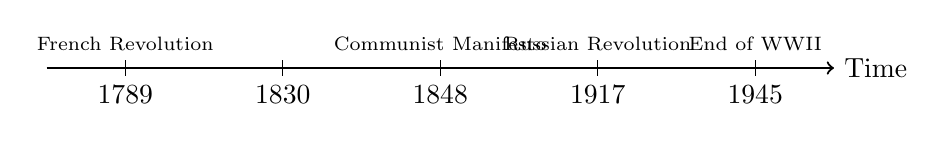
\begin{tikzpicture}
\draw[->, thick] (0,0) -- (10,0) node[right] {Time};
\draw (1,0.1) -- (1,-0.1) node[below] {1789};
\draw (3,0.1) -- (3,-0.1) node[below] {1830};
\draw (5,0.1) -- (5,-0.1) node[below] {1848};
\draw (7,0.1) -- (7,-0.1) node[below] {1917};
\draw (9,0.1) -- (9,-0.1) node[below] {1945};

\node[above] at (1,0.1) {\scriptsize French Revolution};
\node[above] at (5,0.1) {\scriptsize Communist Manifesto};
\node[above] at (7,0.1) {\scriptsize Russian Revolution};
\node[above] at (9,0.1) {\scriptsize End of WWII};
\end{tikzpicture}
\end{center}
\end{frame}

\begin{frame}
\frametitle{Hegel's Dialectic: A New Method of Understanding History}
\begin{itemize}
    \item \textbf{Dialectic} is Hegel's method of understanding how concepts and history develop through contradictions.
    \item The process involves a \textbf{thesis} (initial idea), met by its \textbf{antithesis} (contradiction), resulting in a \textbf{synthesis} (resolution).
    \item This process isn't simply linear but represents the way reality itself unfolds through opposing forces.
    \item For Hegel, contradictions aren't errors in our thinking but essential aspects of reality that drive historical development.
\end{itemize}

\begin{block}{The Dialectical Process}
\begin{center}
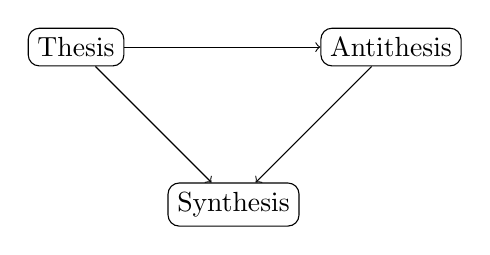
\begin{tikzpicture}
\node[draw, rounded corners] (thesis) at (0,0) {Thesis};
\node[draw, rounded corners] (antithesis) at (4,0) {Antithesis};
\node[draw, rounded corners] (synthesis) at (2,-2) {Synthesis};
\draw[->] (thesis) -- (antithesis);
\draw[->] (thesis) -- (synthesis);
\draw[->] (antithesis) -- (synthesis);
\end{tikzpicture}
\end{center}
\end{block}
\end{frame}

\begin{frame}
\frametitle{The Master-Slave Dialectic: Self-Consciousness Through Others}
\begin{itemize}
    \item In Hegel's famous \textbf{master-slave dialectic}, he shows how self-consciousness requires recognition from others.
    \item The master initially seems independent but paradoxically needs the slave's recognition to confirm his status.
    \item The slave, through work and transforming the world, develops a deeper form of self-consciousness than the master.
    \item This demonstrates Hegel's insight that human identity is inherently social, not individually self-contained.
\end{itemize}

\begin{alertblock}{Key Insight}
The liberal view of individuals as self-sufficient and independent ignores our fundamental need for recognition from others to develop true self-consciousness.
\end{alertblock}
\end{frame}

\begin{frame}
    \frametitle{Case Study: Hegel's Recognition and Master-Slave Dialectic}
    \begin{columns}
    \column{0.6\textwidth}
    \begin{itemize}
        \item \textbf{In The Office:} Michael Scott (regional manager) initially derives self-worth from his title and authority over employees.
        \item His need for employees' recognition reveals his dependence on them for his identity (like Hegel's master).
        \item When Michael leaves to start his own paper company, he develops genuine self-consciousness through productive work and struggle.
        \item Through this dialectical process, Michael evolves beyond needing validation from a position of authority.
    \end{itemize}
    
    \column{0.4\textwidth}
    \begin{alertblock}{Key Hegelian Concepts}
    \begin{itemize}
        \item Recognition from others shapes identity
        \item The paradox of the master's dependence
        \item Self-consciousness through work and struggle
        \item Dialectical process of personal growth
    \end{itemize}
    \end{alertblock}
    \end{columns}
    \end{frame}

\begin{frame}
\frametitle{Ethical Life (Sittlichkeit): Family, Civil Society, and State}
\begin{itemize}
    \item \textbf{Ethical life} (Sittlichkeit) refers to the concrete social institutions that embody freedom in community.
    \item Hegel divides ethical life into three spheres: the \textbf{family} (based on love), \textbf{civil society} (based on self-interest), and the \textbf{state} (based on reason).
    \item Each sphere represents a different way humans experience social belonging and fulfillment.
    \item Unlike liberalism, Hegel sees these institutions not as limiting freedom but as making genuine freedom possible.
\end{itemize}

\begin{center}
\begin{tabular}{p{3cm}p{7cm}}
\toprule
\textbf{Institution} & \textbf{Basis and Function} \\
\midrule
Family & Immediate unity based on love and care \\
Civil Society & Particular interests, market relations, needs \\
State & Universal interest, rational laws, ethical whole \\
\bottomrule
\end{tabular}
\end{center}
\end{frame}

\begin{frame}
    \frametitle{Case Study: Hegel's Ethical Life (Sittlichkeit)}
    \begin{columns}
    \column{0.6\textwidth}
    \begin{itemize}
        \item \textbf{In Star Wars:} The Jedi Order exemplifies Hegel's concept of ethical life with its distinct spheres:
        \item \textbf{Family:} The master-padawan relationship provides immediate bonds of care and mentorship
        \item \textbf{Civil Society:} Jedi interact with the galaxy through particular missions and practical problem-solving
        \item \textbf{State:} The Jedi Council represents universal principles and collective wisdom beyond individual interests
    \end{itemize}
    
    \column{0.4\textwidth}
    \begin{block}{Anakin's Tragedy: A Hegelian View}
    Anakin's fall can be understood as his failure to reconcile these spheres. His attachment to particular relationships (Padmé) conflicts with his universal duties as a Jedi. Instead of finding freedom within the rational structure of the Order, he seeks abstract freedom outside it, leading to his corruption.
    \end{block}
    \end{columns}
    \end{frame}
    

\begin{frame}
\frametitle{The Rational State: Freedom as Recognition}
\begin{itemize}
    \item For Hegel, the \textbf{rational state} is not an oppressive power but the highest expression of freedom.
    \item \textbf{Freedom} for Hegel means being recognized as a person with rights and dignity within a community.
    \item The state should embody reason and universal interests, transcending but preserving both family bonds and market relations.
    \item This contrasts with liberalism's view of the state as a necessary evil that should be limited to protect individual freedom.
\end{itemize}

\begin{exampleblock}{Contrast with Liberal View}
\begin{itemize}
    \item \textbf{Liberal view:} The state limits freedom and should be restricted
    \item \textbf{Hegelian view:} The state enables true freedom through rational institutions
\end{itemize}
\end{exampleblock}
\end{frame}

\begin{frame}
\frametitle{Hegel's Critique of Liberalism: Beyond Abstract Rights}
\begin{itemize}
    \item Hegel criticized liberal rights as too \textbf{abstract} and disconnected from social reality.
    \item He argued that rights only become concrete and meaningful within the context of ethical community.
    \item Merely formal rights (on paper) are empty without the social conditions that make their exercise possible.
    \item By focusing only on individual rights, liberalism fails to address the social conditions necessary for meaningful freedom.
\end{itemize}

\begin{block}{Abstract vs. Concrete Rights}
Consider a right to education: An abstract right merely declares everyone equal before the law, while concrete right requires actual institutions, resources, and social support to make education accessible to all.
\end{block}
\end{frame}

\begin{frame}
\frametitle{History as the Progress of Freedom: The World Spirit}
\begin{itemize}
    \item Hegel viewed history as the progressive realization of human freedom through the development of the \textbf{World Spirit} (Weltgeist).
    \item Each historical epoch represents a stage in humanity's growing self-consciousness and capacity for freedom.
    \item Major historical figures and events are instruments through which the World Spirit advances, often unconsciously.
    \item This teleological view of history contrasts with liberalism's more individualistic and ahistorical approach.
\end{itemize}

\begin{center}
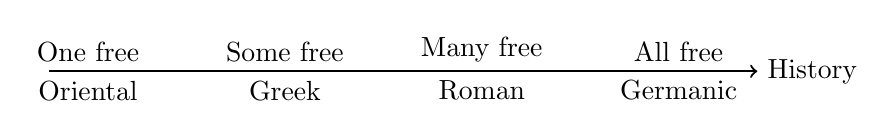
\begin{tikzpicture}
\draw[->, thick] (0,0) -- (9,0) node[right] {History};
\node[below] at (0.5,0) {Oriental};
\node[below] at (3,0) {Greek};
\node[below] at (5.5,0) {Roman};
\node[below] at (8,0) {Germanic};

\node[above] at (0.5,0) {One free};
\node[above] at (3,0) {Some free};
\node[above] at (5.5,0) {Many free};
\node[above] at (8,0) {All free};
\end{tikzpicture}
\end{center}
\end{frame}

\begin{frame}
\frametitle{Hegel's Influence: Setting the Stage for Marx and Beyond}
\begin{itemize}
    \item Hegel's dialectical method was adopted by many subsequent thinkers, especially Marx who "turned it on its head."
    \item His emphasis on history as a meaningful process influenced philosophical approaches to social and political questions.
    \item The concept that freedom requires recognition within community challenged liberal assumptions about autonomy.
    \item Hegel's critique of abstract rights laid groundwork for more socially-embedded conceptions of rights and justice.
\end{itemize}

\begin{alertblock}{The Young Hegelians}
After Hegel's death, a group called the \textbf{Young Hegelians} (including Marx) adopted his dialectical method but rejected his conservative conclusions, applying his approach to criticize existing institutions rather than justify them.
\end{alertblock}
\end{frame}

    
\begin{frame}
\frametitle{Marx's Materialist Turn: From Ideas to Economic Relations}
\begin{itemize}
    \item Marx inverted Hegel's idealism, arguing that material conditions shape ideas rather than the reverse—his \textbf{materialist} approach.
    \item According to Marx, the fundamental reality is not Spirit or ideas but concrete economic relations and productive forces.
    \item \textbf{Materialism} focuses on how humans produce their means of subsistence as the basis of all social life.
    \item This shift makes economic structures, rather than politics or culture, the foundation of social analysis.
\end{itemize}

\begin{exampleblock}{Marx's Materialism vs. Hegel's Idealism}
\begin{center}
\begin{tabular}{ll}
\textbf{Hegel} & Ideas and consciousness determine reality \\
\textbf{Marx} & Material conditions determine consciousness \\
\end{tabular}
\end{center}
"It is not the consciousness of men that determines their being, but, on the contrary, their social being that determines their consciousness." - Marx
\end{exampleblock}
\end{frame}

\begin{frame}
\frametitle{Alienation: The Worker's Estrangement in Capitalism}
\begin{itemize}
    \item \textbf{Alienation} refers to how workers become estranged from their labor, its products, their human nature, and each other under capitalism.
    \item Workers have no control over what they produce or how they produce it, making labor an external, forced activity.
    \item The products of labor belong to the capitalist, standing as alien objects that workers cannot relate to as their own creation.
    \item This contrasts with liberalism's focus on formal freedom while ignoring how economic conditions limit real autonomy.
\end{itemize}

\begin{block}{Four Aspects of Alienation}
\begin{enumerate}
    \item Alienation from the product of labor
    \item Alienation from the act of production
    \item Alienation from human nature (species-being)
    \item Alienation from other humans
\end{enumerate}
\end{block}
\end{frame}

\begin{frame}
    \frametitle{Case Study: Marx's Alienation}
    \begin{columns}
    \column{0.65\textwidth}
    \begin{itemize}
        \item \textbf{In The Simpsons:} Homer Simpson at the Springfield Nuclear Power Plant exemplifies Marx's concept of alienation.
        \item \textbf{From product:} Homer has no connection to the electricity produced or how it's used
        \item \textbf{From process:} His work is repetitive button-pushing disconnected from his human capabilities
        \item \textbf{From species-being:} His creative potential remains unrealized in his mindless labor
        \item \textbf{From others:} Workplace relations are characterized by fear (of Burns) and competition
    \end{itemize}
    
    \column{0.35\textwidth}
    \begin{exampleblock}{Contrast with Non-Alienated Labor}
    When Homer builds his own barbecue pit or invents something in his garage, we see glimpses of non-alienated labor: he controls the process, has a direct relationship with the product, expresses his creativity, and often collaborates with family and friends.
    \end{exampleblock}
    \end{columns}
    \end{frame}
    

\begin{frame}
\frametitle{Historical Materialism: How Economic Systems Shape Society}
\begin{itemize}
    \item \textbf{Historical materialism} is Marx's theory that economic systems and productive relations form the basis of all social structures.
    \item Society's \textbf{economic base} (means of production, relations of production) determines its \textbf{superstructure} (politics, law, culture).
    \item As productive forces develop, they eventually come into conflict with existing relations of production, creating revolutionary situations.
    \item This materialist view challenges liberalism's abstract political theories that ignore economic foundations of social life.
\end{itemize}

\begin{center}
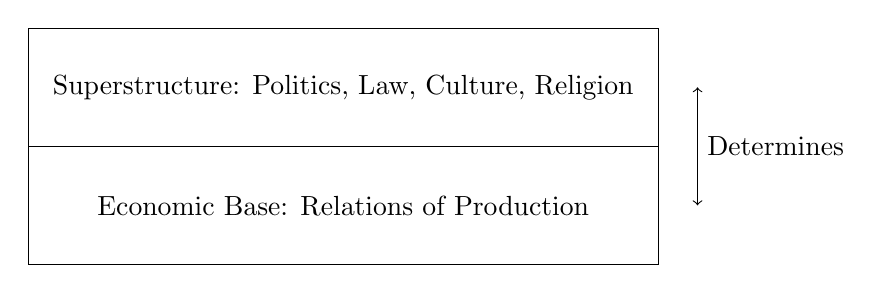
\begin{tikzpicture}
\draw (0,0) rectangle (8,1.5);
\node at (4,0.75) {Superstructure: Politics, Law, Culture, Religion};
\draw (0,0) -- (8,0);
\draw (0,-1.5) rectangle (8,0);
\node at (4,-0.75) {Economic Base: Relations of Production};
\draw[<->] (8.5,0.75) -- (8.5,-0.75) node[midway,right] {Determines};
\end{tikzpicture}
\end{center}
\end{frame}

\begin{frame}
\frametitle{Class Struggle: The Engine of History}
\begin{itemize}
    \item Marx famously declared that "the history of all hitherto existing society is the history of \textbf{class struggles}."
    \item Each economic system creates classes with opposed interests: masters/slaves, lords/serfs, bourgeoisie/proletariat.
    \item Under capitalism, the \textbf{bourgeoisie} (owners of capital) and the \textbf{proletariat} (wage laborers) have fundamentally antagonistic interests.
    \item This conflict ultimately drives historical change, unlike liberalism's focus on individual rights and rational agreement.
\end{itemize}

\begin{alertblock}{Key Historical Transitions}
\begin{tabular}{lll}
\textbf{Economic System} & \textbf{Dominant Classes} & \textbf{Relations} \\
\hline
Primitive Communism & None & Communal ownership \\
Slavery & Masters/Slaves & Ownership of people \\
Feudalism & Lords/Serfs & Land tenure obligations \\
Capitalism & Bourgeoisie/Proletariat & Wage labor \\
Communism & None (classless) & Collective ownership \\
\end{tabular}
\end{alertblock}
\end{frame}

\begin{frame}
\frametitle{Critique of Liberal Rights: Freedom Beyond Formal Equality}
\begin{itemize}
    \item Marx criticized liberal rights as \textbf{formal freedoms} that mask real inequalities and exploitation under capitalism.
    \item The apparent equality before the law obscures the profound economic inequality between workers and capitalists.
    \item Liberal rights like property rights actually serve to protect the interests of the wealthy and powerful.
    \item True human emancipation requires not just political rights but transformation of the economic basis of society.
\end{itemize}

\begin{exampleblock}{Marx on Rights in "On the Jewish Question"}
"None of the supposed rights of man goes beyond the egoistic man, man as he is, as a member of civil society; that is, an individual separated from the community, withdrawn into himself, wholly preoccupied with his private interest and acting in accordance with his private caprice."
\end{exampleblock}
\end{frame}

\begin{frame}
\frametitle{The Communist Vision: From "Each According to Their Ability"}
\begin{itemize}
    \item Marx envisioned communism as a society where exploitation and class division are abolished through collective ownership.
    \item The famous principle "From each according to his ability, to each according to his needs" defines true justice beyond liberal conceptions.
    \item In communist society, alienation would be overcome as people would recognize their labor as a free expression of their humanity.
    \item This vision challenges liberalism's acceptance of capitalism and private property as natural or necessary conditions.
\end{itemize}

\begin{block}{Stages Toward Communist Society}
\begin{enumerate}
    \item Capitalism enters crisis through internal contradictions
    \item Proletarian revolution seizes the means of production
    \item Dictatorship of the proletariat transitions society
    \item Higher phase of communism establishes classless society
\end{enumerate}
\end{block}
\end{frame}

\begin{frame}
\frametitle{Praxis: Philosophy as Active Transformation of Society}
\begin{itemize}
    \item Marx's concept of \textbf{praxis} unites theory and practice, rejecting philosophy that merely interprets the world.
    \item His famous thesis states: "Philosophers have only interpreted the world in various ways; the point, however, is to change it."
    \item This activist orientation challenges the contemplative stance of traditional philosophy, including liberal political theory.
    \item Through praxis, humans simultaneously transform nature, society, and themselves in a unified activity.
\end{itemize}

\begin{center}
\small
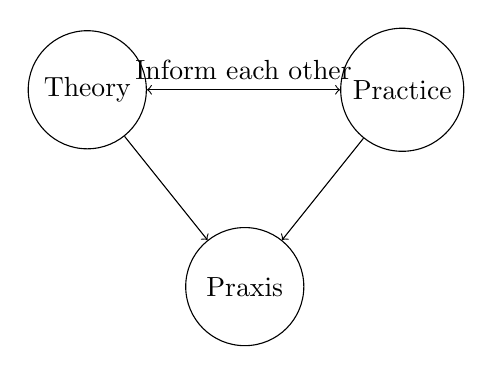
\begin{tikzpicture}
\node[draw, circle, minimum size=1.5cm] (theory) at (0,0) {Theory};
\node[draw, circle, minimum size=1.5cm] (practice) at (4,0) {Practice};
\node[draw, circle, minimum size=1.5cm] (praxis) at (2,-2.5) {Praxis};

\draw[<->] (theory) -- (practice) node[midway, above] {Inform each other};
\draw[->] (theory) -- (praxis);
\draw[->] (practice) -- (praxis);
\end{tikzpicture}
\end{center}
\end{frame}

\begin{frame}
\frametitle{Marx's Legacy: Revolutionary Movements and Critical Theory}
\begin{itemize}
    \item Marx's ideas inspired revolutionary movements across the globe, fundamentally reshaping the political landscape of the 20th century.
    \item His analysis of capitalism continues to provide tools for understanding economic exploitation and inequality.
    \item Critical theory, feminism, postcolonial theory, and other modern schools of thought draw extensively on Marxist concepts.
    \item The failure of actually existing socialism raises important questions about Marx's vision while not invalidating his critique.
\end{itemize}

\begin{alertblock}{Critical Evaluation}
While Marx's predictions about capitalism's collapse have not fully materialized, his insights about alienation, commodification, and economic inequality remain powerful tools for social critique in the 21st century.
\end{alertblock}
\end{frame}


\begin{frame}
\frametitle{Hannah Arendt: Political Thought After Totalitarianism}
\begin{itemize}
    \item \textbf{Hannah Arendt} developed her political theory in response to the unprecedented horrors of totalitarianism in the 20th century.
    \item Unlike Marx, she was skeptical of deterministic views of history and emphasized the unpredictability of human action.
    \item Arendt sought to recover the dignity of politics as a distinct sphere of human freedom and plurality.
    \item Her work represents a third alternative to both liberalism's individualism and Marxism's economic determinism.
\end{itemize}

\begin{exampleblock}{Biographical Context}
Arendt (1906-1975) was a German-Jewish philosopher who fled Nazi Germany in 1933. Her experiences as a refugee and her observations of totalitarianism profoundly shaped her political thinking about the fragility of the public realm and the dangers of mass society.
\end{exampleblock}
\end{frame}

\begin{frame}
\frametitle{The Human Condition: Labor, Work, and Action}
\begin{itemize}
    \item In "The Human Condition," Arendt distinguishes three fundamental human activities: \textbf{labor}, \textbf{work}, and \textbf{action}.
    \item \textbf{Labor} is the activity that corresponds to biological necessity and sustains life itself.
    \item \textbf{Work} creates the artificial world of durable objects, providing stability and permanence.
    \item \textbf{Action} is specifically political activity through which we reveal our unique identities in the public realm.
\end{itemize}

\begin{center}
\begin{tabular}{lll}
\toprule
\textbf{Activity} & \textbf{Purpose} & \textbf{Character} \\
\midrule
Labor & Biological survival & Cyclical, never-ending \\
Work & Creating durability & Instrumental, means-end \\
Action & Revealing who we are & Unpredictable, revelatory \\
\bottomrule
\end{tabular}
\end{center}
\end{frame}

\begin{frame}
\frametitle{The Public Realm: Politics as Collective Appearance}
\begin{itemize}
    \item For Arendt, the \textbf{public realm} is a space of appearance where individuals reveal themselves through speech and action.
    \item Politics is not primarily about governing or distributing resources but about creating a common world through collective deliberation.
    \item The public sphere has been endangered by both totalitarianism and consumer society, which reduce humans to mere specimens.
    \item This view contrasts with liberalism's focus on privacy and with Marx's emphasis on economics over politics.
\end{itemize}

\begin{block}{Public vs. Private Realms}
Arendt draws on the ancient Greek distinction between the \textit{polis} (public realm of freedom and equality) and the \textit{oikos} (household realm of necessity and hierarchy), arguing that modern society has created a problematic "social" realm that confuses these boundaries.
\end{block}
\end{frame}

\begin{frame}
\frametitle{Natality: The Capacity for New Beginnings}
\begin{itemize}
    \item \textbf{Natality}—the fact of being born—is central to Arendt's political thought as the capacity to begin something new.
    \item Each birth represents the arrival of someone who has never existed before and who can initiate unpredictable action.
    \item This emphasis on new beginnings counters deterministic views of history (whether liberal progress or Marxist historical materialism).
    \item Natality provides hope against totalitarianism's attempt to eliminate human spontaneity and unpredictability.
\end{itemize}

\begin{alertblock}{Against Determinism}
"The miracle that saves the world, the realm of human affairs, from its normal, 'natural' ruin is ultimately the fact of natality, in which the faculty of action is ontologically rooted."
\end{alertblock}
\end{frame}

\begin{frame}
    \frametitle{Case Study: Arendt's Natality and Action}
    \begin{columns}
        \small
    \column{0.6\textwidth}
    \begin{itemize}
        \item \textbf{In Toy Story:} The toys' secret lives illustrate Arendt's concepts of natality and action.
        \item Woody and Buzz initiate new, unpredictable beginnings when they act in ways their design never anticipated
        \item Their actions create a plural community where each toy reveals their unique identity
        \item Their adventures demonstrate the unpredictability of action—how initiatives set in motion consequences that cannot be controlled
        \item The contrast between being treated as objects (mere things) and acting as subjects who create meaning
    \end{itemize}
    
    \column{0.4\textwidth}
    \begin{exampleblock}{Arendtian Moments}
    When Woody calls the toys to a staff meeting, he creates a public space for speech and action. Each toy appears before others, revealing who they are beyond what they are. The difference between how toys behave when humans are present (labor/survival) versus when they're alone (political action) parallels Arendt's distinction between necessity and freedom.
    \end{exampleblock}
    \end{columns}
    \end{frame}

\begin{frame}
\frametitle{Power vs. Violence: Rethinking Political Force}
\begin{itemize}
    \item Arendt makes a crucial distinction between \textbf{power} and \textbf{violence} that challenges traditional political thinking.
    \item \textbf{Power} emerges when people act together and is essentially communicative and consensual.
    \item \textbf{Violence} is instrumental and can destroy power but can never create it or substitute for it.
    \item This reframes politics away from domination (whether liberal or Marxist) toward collective capacity for action.
\end{itemize}

\begin{center}
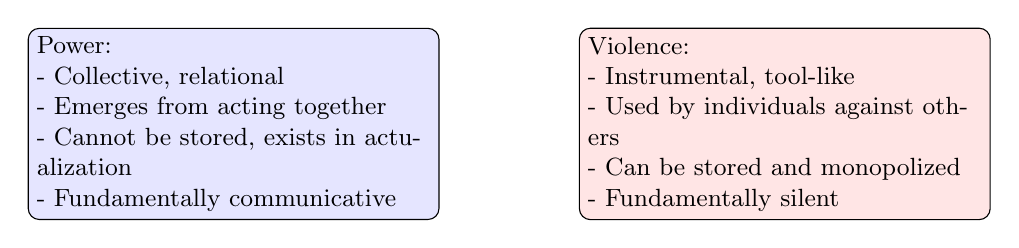
\begin{tikzpicture}
\small
\node[draw, rounded corners, fill=blue!10, text width=5cm] at (0,0) 
    {Power:\\
    - Collective, relational\\
    - Emerges from acting together\\
    - Cannot be stored, exists in actualization\\
    - Fundamentally communicative};
    
\node[draw, rounded corners, fill=red!10, text width=5cm] at (7,0) 
    {Violence:\\
    - Instrumental, tool-like\\
    - Used by individuals against others\\
    - Can be stored and monopolized\\
    - Fundamentally silent};
\end{tikzpicture}
\end{center}
\end{frame}

\begin{frame}
\frametitle{The Banality of Evil: Thoughtlessness in Modern Society}
\begin{itemize}
    \item Arendt's concept of the \textbf{banality of evil} emerged from her observation of Nazi officer Adolf Eichmann at his trial.
    \item Evil can result not from monstrous hatred but from ordinary thoughtlessness and failure to reflect on one's actions.
    \item Modern bureaucracy and technical efficiency can discourage thinking and judgment, facilitating moral catastrophes.
    \item This understanding challenges both liberal faith in rational progress and Marxist focus on class interest as explanations for political behavior.
\end{itemize}

\begin{exampleblock}{Eichmann in Jerusalem}
"The trouble with Eichmann was precisely that so many were like him, and that the many were neither perverted nor sadistic, that they were, and still are, terribly and terrifyingly normal."
\end{exampleblock}
\end{frame}

\begin{frame}
\frametitle{Plurality: The Condition of Human Action}
\begin{itemize}
    \item \textbf{Plurality}—the fact that humans are both equal and distinct—is for Arendt the fundamental condition of political life.
    \item Political action requires others who are sufficiently similar to understand us yet different enough to make communication meaningful.
    \item Totalitarianism attempts to eliminate plurality by reducing humans to interchangeable members of a species or class.
    \item This emphasis on irreducible human distinctness challenges both liberalism's abstract individual and Marxism's class-based analysis.
\end{itemize}

\begin{block}{The Paradox of Plurality}
Plurality contains a dual character: equality (without which we could not understand each other) and distinction (without which we would not need speech and action to make ourselves understood).
\end{block}
\end{frame}

\begin{frame}
\frametitle{Arendt's Critique of Marx: The Dangers of Historical Necessity}
\begin{itemize}
    \item Arendt criticized Marx for subordinating politics to economics and for his deterministic view of historical development.
    \item She warned that Marx's elevation of labor risked reducing humans to mere animal laborans, concerned only with biological necessity.
    \item Marx's focus on historical necessity could justify violence and undermine the unpredictability essential to genuine political action.
    \item Despite these critiques, Arendt shared Marx's concern with the impact of economic conditions on human freedom.
\end{itemize}

\begin{alertblock}{Labor vs. Action}
For Arendt, Marx's emphasis on labor misses the unique human capacity for action that transcends necessity. She feared that the "glorification of labor" in Marxism might inadvertently contribute to reducing humans to their biological functions.
\end{alertblock}
\end{frame}


\begin{frame}
\frametitle{Challenging Individual Rights: Communal Alternatives to Liberalism}
\begin{itemize}
    \item All three thinkers challenge liberalism's focus on abstract individual rights as the foundation of political philosophy.
    \item Hegel sees rights as meaningful only within ethical communities that provide recognition and concrete substance.
    \item Marx views liberal rights as masking economic exploitation and serving the interests of the ruling class.
    \item Arendt argues that rights require a political community and can become meaningless when people are reduced to "mere humans."
\end{itemize}

\begin{center}
\begin{tabular}{lp{8cm}}
\toprule
\textbf{Thinker} & \textbf{Critique of Liberal Rights} \\
\midrule
Hegel & Rights require social recognition and institutional embodiment \\
Marx & Rights obscure class exploitation and protect property interests \\
Arendt & Rights depend on citizenship in a political community \\
\bottomrule
\end{tabular}
\end{center}
\end{frame}

\begin{frame}
\frametitle{Freedom Reconceived: Beyond Negative Liberty}
\begin{itemize}
    \item Liberalism primarily conceives of \textbf{freedom as negative liberty}—freedom from interference by others or the state.
    \item Hegel redefines freedom as \textbf{recognition} within a rational community that makes self-realization possible.
    \item Marx understands true freedom as \textbf{non-alienated labor} in a society where economic exploitation has been abolished.
    \item Arendt sees freedom as the capacity for \textbf{political action} that creates new beginnings within a plural public realm.
\end{itemize}

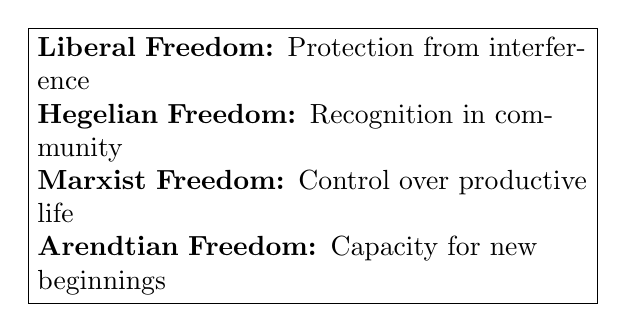
\begin{tikzpicture}
\node[draw, text width=7cm] at (4,0) {
\textbf{Liberal Freedom:} Protection from interference\\
\textbf{Hegelian Freedom:} Recognition in community\\
\textbf{Marxist Freedom:} Control over productive life\\
\textbf{Arendtian Freedom:} Capacity for new beginnings
};
\end{tikzpicture}
\end{frame}

\begin{frame}
\frametitle{The Role of the State: From Necessary Evil to Ethical Community}
\begin{itemize}
    \item Liberalism views the \textbf{state} primarily as a necessary evil that should be limited to protect individual rights.
    \item For Hegel, the rational state is the highest embodiment of ethical life and the actualization of freedom.
    \item Marx sees the state under capitalism as a tool of class oppression that will eventually wither away in communist society.
    \item Arendt distinguishes political power from state governance, emphasizing the public realm over administrative functions.
\end{itemize}

\begin{block}{Beyond Liberal Statecraft}
While liberalism treats politics primarily as a means to protect pre-political private interests, these thinkers see political life as having intrinsic value and importance for human fulfillment.
\end{block}
\end{frame}

\begin{frame}
\frametitle{Relevance Today: How These Thinkers Help Us Understand Modern Politics}
\begin{itemize}
    \item Hegel's emphasis on \textbf{recognition} helps us understand identity politics and contemporary struggles for dignity.
    \item Marx's analysis of \textbf{economic power} illuminates growing inequality and the political influence of corporations.
    \item Arendt's concern with the \textbf{public realm} speaks to the challenges of maintaining democratic discourse in digital society.
    \item Together, they provide resources for critiquing neoliberalism's narrowing of political possibilities to market logic.
\end{itemize}

\begin{exampleblock}{Contemporary Applications}
\begin{itemize}
    \item Social media and Arendt's public realm
    \item Automation and Marx's alienation
    \item The politics of recognition for marginalized groups
    \item Consumer identity vs. political identity
\end{itemize}
\end{exampleblock}
\end{frame}

\begin{frame}
\frametitle{Critical Questions: Strengths and Weaknesses of Post-Liberal Thought}
\begin{itemize}
    \item Can Hegel's rational state avoid becoming authoritarian by claiming to embody universal reason?
    \item Does Marx's focus on economic relations adequately account for non-class-based forms of oppression and identity?
    \item Is Arendt's sharp distinction between political action and social/economic issues sustainable in modern society?
    \item How can we incorporate these critiques of liberalism without abandoning crucial protections for individual rights?
\end{itemize}

\begin{alertblock}{Beyond the Individual: The Continuing Challenge to Liberalism}
The enduring insight from these thinkers is that genuine human freedom cannot be understood in purely individualistic terms but requires attention to the social, economic, and political conditions that make meaningful freedom possible.
\end{alertblock}
\end{frame}

\end{document}